\begin{table}[h!]
\centering
\caption{Detalhamento dos modelos obtidos com a arquitetura ShuffleNet para cada uma das abordagens consideradas neste trabalho.}
\label{tab:shufflenet}
\resizebox{\textwidth}{!}{\begin{tabular}{ccccccc}
\toprule
\textbf{Abordagem} & \textbf{Otimizador} & \textbf{\emph{Patience}}  & \textbf{Função de Ativação} & \textbf{Acurácia} & \textbf{F-Score} & \textbf{EER} \\
\midrule
Abordagem A & RMSprop & 15 & ReLU & $0.9404$ & $0.9004$ & $7.5400$ \\
Abordagem B & RMSprop & 15 & ReLU & $0.8345$ & $0.7705$ & $23.8151$\\
\bottomrule
\end{tabular}}
\end{table}
    
\begin{figure}[H]
\centering
\caption{Histórico de \emph{loss} e acurácia durante o treinamento dos modelos obtidos com a arquitetura ShuffleNet.}
\label{fig:treinamento-shufflenet}
\subfloat[\emph{Loss} durante treinamento da rede ShuffleNet para a abordagem A.\label{subfig:shufflenet-a-loss}]{%
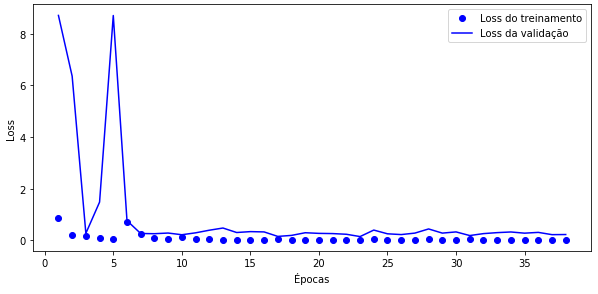
\includegraphics[width=0.47\textwidth]{imgs/shufflenet-a-loss}
}
\hfill
\subfloat[Acurácia durante treinamento da rede ShuffleNet para a abordagem A.\label{subfig:shufflenet-a-acc}]{%
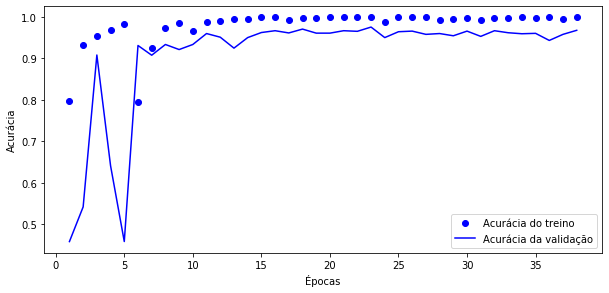
\includegraphics[width=0.47\textwidth]{imgs/shufflenet-a-acc}
}
\hfill
\subfloat[\emph{Loss} durante treinamento da rede ShuffleNet para a abordagem B.\label{subfig:shufflenet-b-loss}]{%
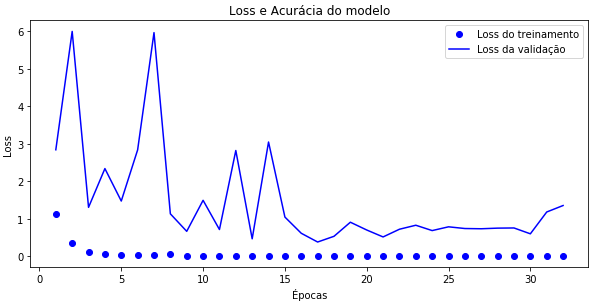
\includegraphics[width=0.47\textwidth]{imgs/shufflenet-b-loss}
}
\hfill
\subfloat[Acurácia durante treinamento da rede ShuffleNet para a abordagem B.\label{subfig:shufflenet-b-acc}]{%
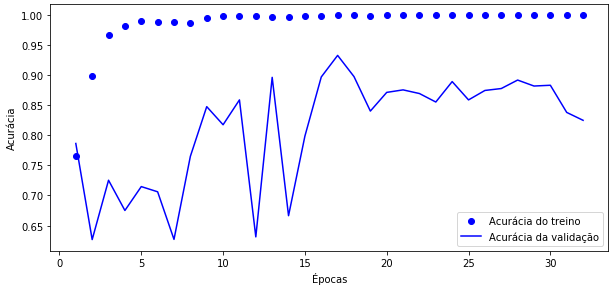
\includegraphics[width=0.47\textwidth]{imgs/shufflenet-b-acc}
}
\end{figure}
    
\begin{figure}[h]
    \centering
    \caption{Matrizes de confusão dos modelos obtidos com a arquitetura ShuffleNet.}\label{fig:matrizes-shufflenet}
    \subfloat[ShuffleNet com a abordagem A\label{subfig:matriz-shufflenet-a}]{%
    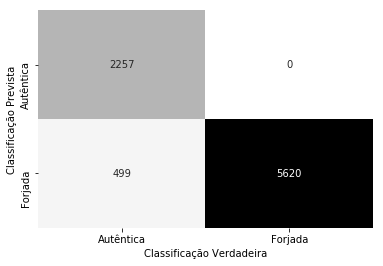
\includegraphics[width=0.47\textwidth]{imgs/matriz-shufflenet-a}
    }
    \hfill
    \subfloat[ShuffleNet com a abordagem B\label{subfig:matriz-shufflenet-b}]{%
    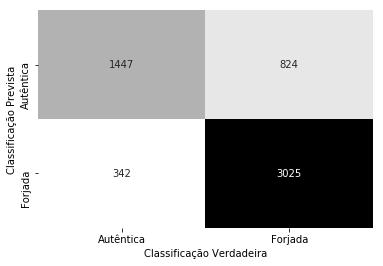
\includegraphics[width=0.47\textwidth]{imgs/matriz-shufflenet-b}
    }
\end{figure}